% Nine panels in a 3x3 grid: scan left-to-right, top-to-bottom.
% Rows: (1) classical distances / similarity, (2) extrema + sparsity metrics,
%       (3) intrinsic fingerprint + two reserved slots for upcoming metrics.
\begin{figure*}[!t]
    \centering
    % --- row 1 ---
    \begin{subfigure}{0.32\textwidth}
        \centering
        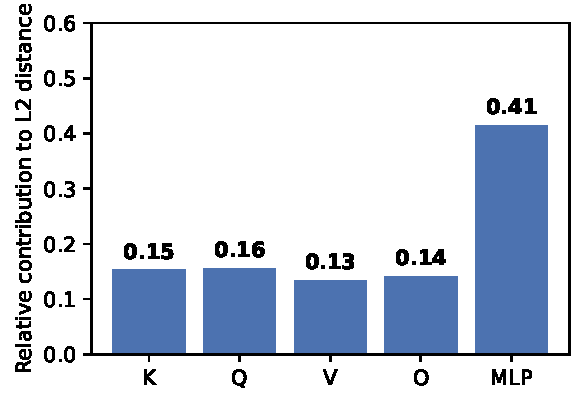
\includegraphics[width=\textwidth]{fig/rq2_l2_layer_contrib.pdf}
        \caption{$L_2$ Distance}
        \label{fig:rq2-l2-layer-contrib}
    \end{subfigure}%
    \hfill
    \begin{subfigure}{0.32\textwidth}
        \centering
        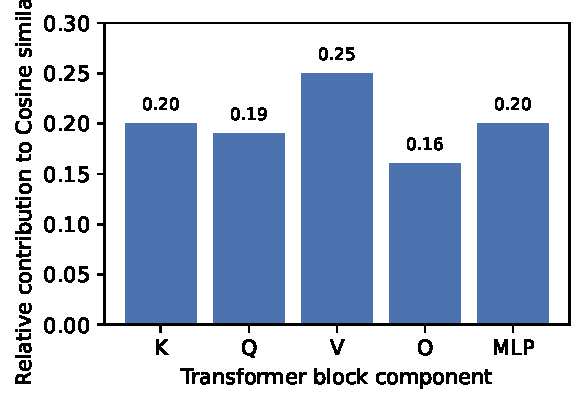
\includegraphics[width=\textwidth]{fig/rq2_cos_layer_contrib.pdf}
        \caption{Cosine Similarity}
        \label{fig:rq2-cos-layer-contrib}
    \end{subfigure}%
    \hfill
    \begin{subfigure}{0.32\textwidth}
        \centering
        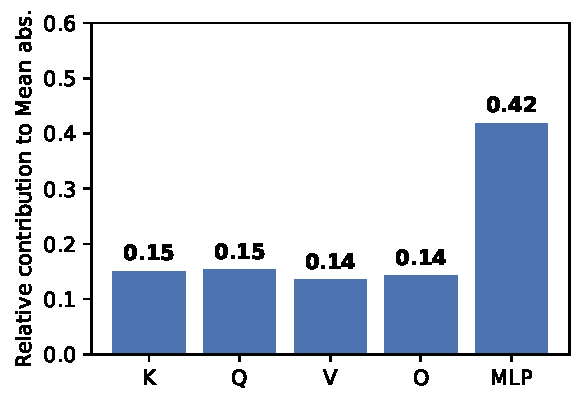
\includegraphics[width=\textwidth]{fig/rq2_abs_mean_layer_contrib.pdf}
        \caption{Abs Mean}
        \label{fig:rq2-abs-mean-layer-contrib}
    \end{subfigure}

    \vspace{0.3cm}

    % --- row 2 ---
    \begin{subfigure}{0.32\textwidth}
        \centering
        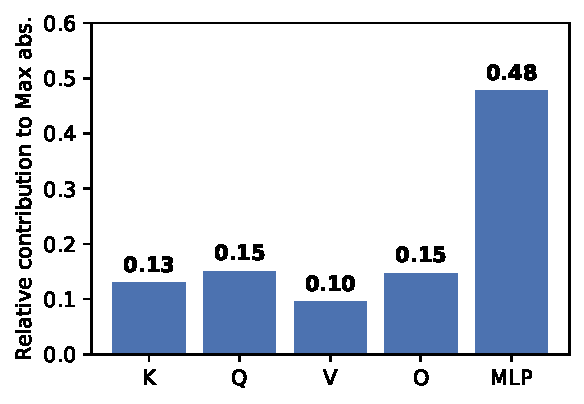
\includegraphics[width=\textwidth]{fig/rq2_abs_max_layer_contrib.pdf}
        \caption{Abs Max}
        \label{fig:rq2-abs-max-layer-contrib}
    \end{subfigure}%
    \hfill
    \begin{subfigure}{0.32\textwidth}
        \centering
        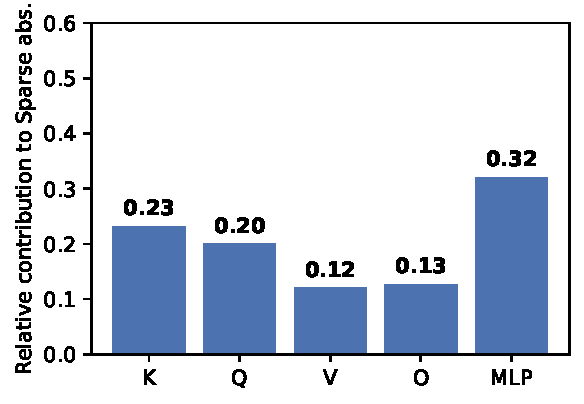
\includegraphics[width=\textwidth]{fig/rq2_sparse_abs_layer_contrib.pdf}
        \caption{Sparse Abs.}
        \label{fig:rq2-sparse-abs-layer-contrib}
    \end{subfigure}%
    \hfill
    \begin{subfigure}{0.32\textwidth}
        \centering
        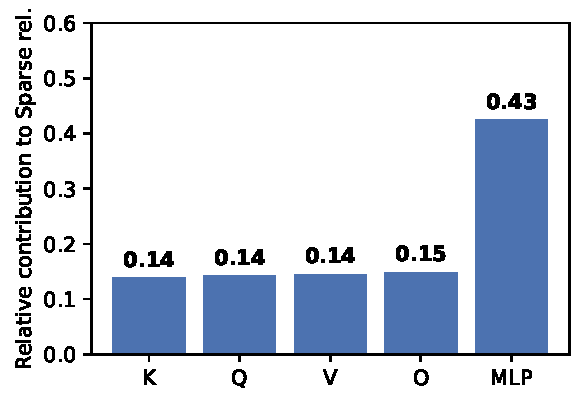
\includegraphics[width=\textwidth]{fig/rq2_sparse_rel_layer_contrib.pdf}
        \caption{Sparse Rel.}
        \label{fig:rq2-sparse-rel-layer-contrib}
    \end{subfigure}

    \vspace{0.3cm}

    % --- row 3 ---
    \begin{subfigure}{0.32\textwidth}
        \centering
        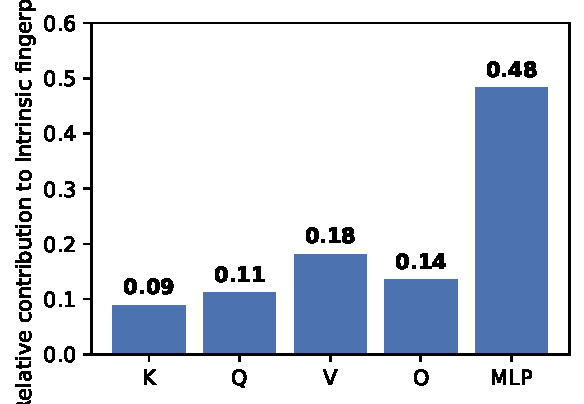
\includegraphics[width=\textwidth]{fig/rq2_intrinsic_fingerprint_layer_contrib.pdf}
        \caption{Intrinsic Fingerprint}
        \label{fig:rq2-intrinsic-fingerprint-layer-contrib}
    \end{subfigure}%
    \hfill
    \begin{subfigure}{0.32\textwidth}
        \centering
        \fbox{%
            \begin{minipage}[c][0.26\textwidth][c]{\dimexpr\textwidth-2\fboxsep-2\fboxrule}
                \centering
                \textcolor{gray}{\small\textit{Placeholder (metric to be added)}}
            \end{minipage}%
        }
        \caption{\textit{Matrix}}
        \label{fig:rq2-layer-contrib-placeholder-a}
    \end{subfigure}%
    \hfill
    \begin{subfigure}{0.32\textwidth}
        \centering
        \fbox{%
            \begin{minipage}[c][0.26\textwidth][c]{\dimexpr\textwidth-2\fboxsep-2\fboxrule}
                \centering
                \textcolor{gray}{\small\textit{Placeholder (metric to be added)}}
            \end{minipage}%
        }
        \caption{\textit{HuRef}}
        \label{fig:rq2-layer-contrib-placeholder-b}
    \end{subfigure}

    \caption{Contribution of different transformer block components (K/Q/V/O/MLP) to various distance metrics (RQ2).}
    \label{fig:rq2-all-metrics-layer-contrib}
\end{figure*}
